% Copyright 2006 by Till Tantau
%
% This file may be distributed and/or modified
%
% 1. under the LaTeX Project Public License and/or
% 2. under the GNU Free Documentation License.
%
% See the file doc/generic/pgf/licenses/LICENSE for more details.


\section{Transparency}

\label{section-transparency}


\begin{package}{pgfbasetransparency}
  This package provides commands for specifying how transparent
  objects are. The package is loaded automatically by 
  |pgf|, but you can load it manually if you have only included
  |pgfcore|.   
\end{package}


\subsection{Overview}

Normally, when you paint something using any of \pgfname's commands
(this includes stroking, filling, shading, patterns, and images), the
newly painted objects totally obscure whatever was painted earlier in
the same area.

You can change this behaviour by using something that can be thought
of as ``(semi)transparent colors.'' Such colors do not completely
obscure the background, rather they blend the background with the new
color. At first sight, using such semitransparent colors might seem quite
straightforward, but the math going on in the background is quite
involved and the correct handling of transparency fills some 64 pages
in the PDF specification. 

In the present section, we start with the different ways of specifying
``how transparent'' newly drawn objects should be. The simplest way is
to just specify a percentage like ``60\% transparent.'' A much more
general way is to use something that I call a \emph{fading,} also
known as a soft mask or a mask. Finally, it is possible to use an
image to specify such a mask in a special way.

At the end of the section we adress the problem of creating so-called
\emph{transparency groups}. This problem arises when you paint over a
position several times with a semitransparent color. Sometimes you
want the effect to accumulate, sometimes you do not.


\emph{Note:} Transparency is best supported by the pdf\TeX\
driver. The \textsc{svg} driver also has some support. For PostScript
output, opacity is rendered correctly only with the most recent
versions of GhostScript. Printers and other programs will typically
ignore the opacity setting. 


\subsection{Specifying a Uniform Opacity}

Specifying a stroke and/or fill opacity is quite easy.

\begin{command}{\pgfsetstrokeopacity\marg{value}}
  Sets the opacity of stroking operations. The \meta{value} should be
  a number between |0| and |1|, where |1| means ``fully opaque'' and
  |0| means ``fully transparent.'' A value like |0.5| will cause paths
  to be stroked in a semitransparent way.
  
\begin{codeexample}[]
\begin{pgfpicture}
  \pgfsetlinewidth{5mm}
  \color{red}
  \pgfpathcircle{\pgfpoint{0cm}{0cm}}{10mm} \pgfusepath{stroke}
  \color{black}
  \pgfsetstrokeopacity{0.5}
  \pgfpathcircle{\pgfpoint{1cm}{0cm}}{10mm} \pgfusepath{stroke}
\end{pgfpicture}
\end{codeexample}
\end{command}


\begin{command}{\pgfsetfillopacity\marg{value}}
  Sets the opacity of filling operations. As for stroking, the
  \meta{value} should be a number between |0| and~|1|.

  The ``filling transparency'' will also be used for text and images.  
  
\begin{codeexample}[]
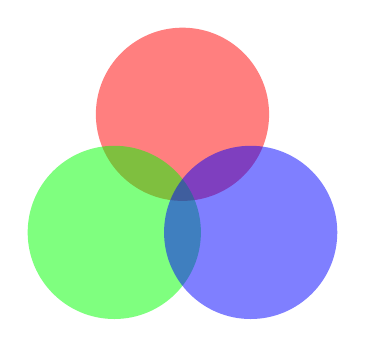
\begin{tikzpicture}
  \pgfsetfillopacity{0.5}
  \fill[red]   (90:1cm)  circle (11mm);
  \fill[green] (210:1cm) circle (11mm);
  \fill[blue]  (-30:1cm) circle (11mm);
\end{tikzpicture}
\end{codeexample}
\end{command}

Note the following effect: If you setup a certain opacity for stroking
or filling and you stroke or fill the same area twice, the effect
accumulates:

\begin{codeexample}[]
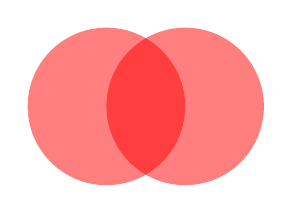
\begin{tikzpicture}
  \pgfsetfillopacity{0.5}
  \fill[red] (0,0) circle (1);
  \fill[red] (1,0) circle (1);
\end{tikzpicture}
\end{codeexample}

Often, this is exactly what you intend, but not always. You can use
transparency groups, see the end of this section, to change this.



\subsection{Transparency Groups}

Consider the following cross and sign. They ``look wrong'' because we
can see how they were constructed, while this is not really part of
the desired effect. 

\begin{codeexample}[]

\begin{tikzpicture}
  \pgfsetstrokeopacity{0.5}
  \draw [line width=5mm] (0,0) -- (2,2);
  \draw [line width=5mm] (2,0) -- (0,2);
\end{tikzpicture}
\end{codeexample}

\begin{codeexample}[]
\begin{tikzpicture}
  \node at (0,0) [forbidden sign,line width=2ex,draw=red,fill=white] {Smoking};
  \pgfsetstrokeopacity{0.5}
  \pgfsetfillopacity{0.5}
  \node at (2,0) [forbidden sign,line width=2ex,draw=red,fill=white] {Smoking};
\end{tikzpicture}
\end{codeexample}

Transparency groups are used to render them correctly:

\begin{codeexample}[]

\begin{tikzpicture}
  \pgfsetfillopacity{0.5}
  \pgftransparencygroup
    \draw [line width=5mm] (0,0) -- (2,2);
    \draw [line width=5mm] (2,0) -- (0,2);
  \endpgftransparencygroup
\end{tikzpicture}
\end{codeexample}

\begin{codeexample}[]
\begin{tikzpicture}
  \node at (0,0) [forbidden sign,line width=2ex,draw=red,fill=white] {Smoking};
  \pgfsetfillopacity{0.5}
  \pgftransparencygroup
    \node at (2,0) [forbidden sign,line width=2ex,draw=red,fill=white]
      {Smoking};
  \endpgftransparencygroup
\end{tikzpicture}
\end{codeexample}





%%% Local Variables: 
%%% mode: latex
%%% TeX-master: "pgfmanual"
%%% End: 
